% !TeX root = ../thuthesis-example.tex

\chapter{可预测预训练--超参数可预测扩展}

% \pkg{natbib} 


在上一章中,我总体介绍了预训练技术以及可预测预训练技术的理念。在本章中,我将介绍本文可预测预训练技术的第一部分,即超参数可预测扩展技术。

\section{预训练超参数简介}

在深度学习模型的预训练中,超参数起着关键作用,直接影响模型的训练效率、性能表现以及最终的泛化能力。

\paragraph{参数初始化方案}
参数初始化是模型训练的起点,合理的初始化方案能够加速模型收敛,避免梯度消失或梯度爆炸等问题。常见的初始化方法包括随机初始化和基于特定分布的初始化。随机初始化通常是从均匀分布或正态分布中随机采样数值来初始化模型参数。例如,在神经网络中,权重矩阵可以通过均匀分布初始化,使每个参数在一定范围内取值,这有助于打破模型训练的对称性,防止所有神经元在训练过程中表现一致。
另一种常用的初始化方法是基于特定分布的初始化,如 Xavier初始化~\cite{pmlr-v9-glorot10a}和 He初始化~\cite{he2015delving}。Xavier初始化根据输入和输出神经元的数量来调整初始化参数的标准差,使得在正向传播和反向传播过程中,信号能够在各层之间较为均匀地传递,从而提高训练的稳定性。He 初始化则针对 ReLU 激活函数进行了优化,它能够更好地适应 ReLU 函数在负半轴输出为 0 的特性,使得模型在使用 ReLU 激活函数时能够更快地收敛。
在本章中,我们对参数初始化方案进行了调整,主要参考来自Tensor Program的初始化方案,结合实际大语言模型训练的实际情况,实现稳定的规模化。


\paragraph{批量大小(batch size)}
批量大小指的是在一次训练迭代中,用于计算梯度和更新参数的样本数量。较大的批量大小可以利用更多的数据信息来计算梯度,使得梯度估计更加准确,从而加速模型的收敛。然而,较大的批量大小也会带来更高的内存需求和计算成本,并且可能导致模型在训练过程中对某些样本的过拟合。
较小的批量大小可以在每次迭代中更快地更新参数,增加模型训练的随机性,有助于跳出局部最优解。但同时,由于每次使用的数据量较少,梯度估计的噪声较大,可能会导致模型收敛不稳定。在传统深度学习的训练中,需要根据数据集的大小、模型的复杂度以及硬件资源等因素来选择合适的批量大小。通常,可以通过实验来探索不同批量大小对模型性能的影响,从而找到最优的设置。然而在大语言模型训练中,没有办法在每次大规模实验前仔细调整批量大小,因此研究批量大小如何随着模型规模扩大变得很重要。

\paragraph{学习率}
学习率决定了模型在训练过程中参数更新的步长。如果学习率设置过小,模型的训练过程会非常缓慢,需要更多的训练轮次才能达到较好的收敛效果;而如果学习率设置过大,模型可能会在训练过程中无法收敛,甚至出现损失函数不断增大的情况。
常见的学习率调整策略包括固定学习率、学习率衰减和自适应学习率。固定学习率在整个训练过程中保持不变,适用于一些简单的模型和数据集。学习率衰减则是在训练过程中逐渐降低学习率,这样可以在训练初期快速更新参数,加速收敛,而在训练后期减小步长,避免错过最优解。常见的学习率衰减方法有指数衰减、余弦退火衰减等。在模型规模扩大过程做,最优的学习率不是通常不是一成不变的。在本章中,我们将结合多方调整,使最优学习率保持稳定。

\improvement{加一个Transformer图}

\section {参数初始化设置}
Tensor Program\citep{yang2022tensor, yang2023tensor} 提出了一个框架,用于稳定不同规模模型的超参数。Tensor Program 的主要部分是宽度缩放\citep{yang2022tensor} 和深度缩放\citep{yang2023tensor}。前者帮助 CerebrasGPT~\citep{dey2023cerebras} 更准确地预测大语言模型的损失。我们对这些技术进行了广泛尝试,有选择地使用了其中几种作为最终方案。

这些操作包括
\begin{enumerate}
  \item 嵌入层输出缩放:将嵌入层的输出乘以$\text{scale\_\text{emb}}$。
  \item 残差连接缩放:在将每个层的块的输出张量添加到每个残差连接之前,将其按$\text{scale\_\text{depth}}/\sqrt{\text{num\_layers}}$进行缩放。
  \item 张量初始化:将每个二维张量参数的初始化标准差设置为$\text{init\_std}/\sqrt{d_m/d_{base}}$,并将其他参数的初始化设置为0.1。
  \item 张量的学习率缩放:将每个二维张量参数的学习率调整为其他部分(或整体学习率)学习率的$1/({d_m/d_{base}})$倍。
  \item 语言模型头部缩放:将输出的对数几率调整为原始值的$1/(d_m/d_{base})$倍。
\end{enumerate}

由于在大语言模型的实际应用中,多注意力头的维度一般为64维,或者128维,而只会方法多注意力头的个数,因此处于这点考虑,本文没有应用~\citep{yang2022tensor} 中提出的注意力Softmax操作归一化因子的缩放技术技术。

与\cite{yang2023tensor}中不同之处在于,他们提出,对于深度大于 2 的网络,深度缩放并不令人满意,但我们通过实验发现得到的最优学习率是稳定的。

\subsection{贝叶斯超参数搜索}
该超参数的扩展方案进一步引入了三个模型大小无关超参数,为了确定这三个超参数,我们在一组预定义的参数空间上进行了广泛的贝叶斯搜索。我们针对 $N = 0.009B$ 的模型进行搜索。为了进一步减少实验需要的资源,在前期实验中,我们证实,当使用规模为 $10N$ 和 $20N$ 数量级的数据集进行超参数优化时,超参数的有效性呈现出一致性。因此,我们使用 $|D| = 10N = 0.09B$ 个词元(tokens)来训练模型。

同时,我们还尝试了QK - Norm~\citep{henry-etal-2020-query}和独立权重衰减~\citep{loshchilov2017decoupled},以稳定学习率。整体结果如图\ref{fig:mupsearch_app}所示。应用QK-norm后,我们观察到学习率敏感性显著降低,这与~\cite{wortsman2023small}的情况类似。根据图\ref{fig:mupsearch_app}中,我们确定了最佳超参数为 $scale\_depth = 1.4$,$scale\_emb = 12$,$init\_std = 0.1$ 以及 $lr = 0.01$。


\begin{figure}[htbp]
  \centering
  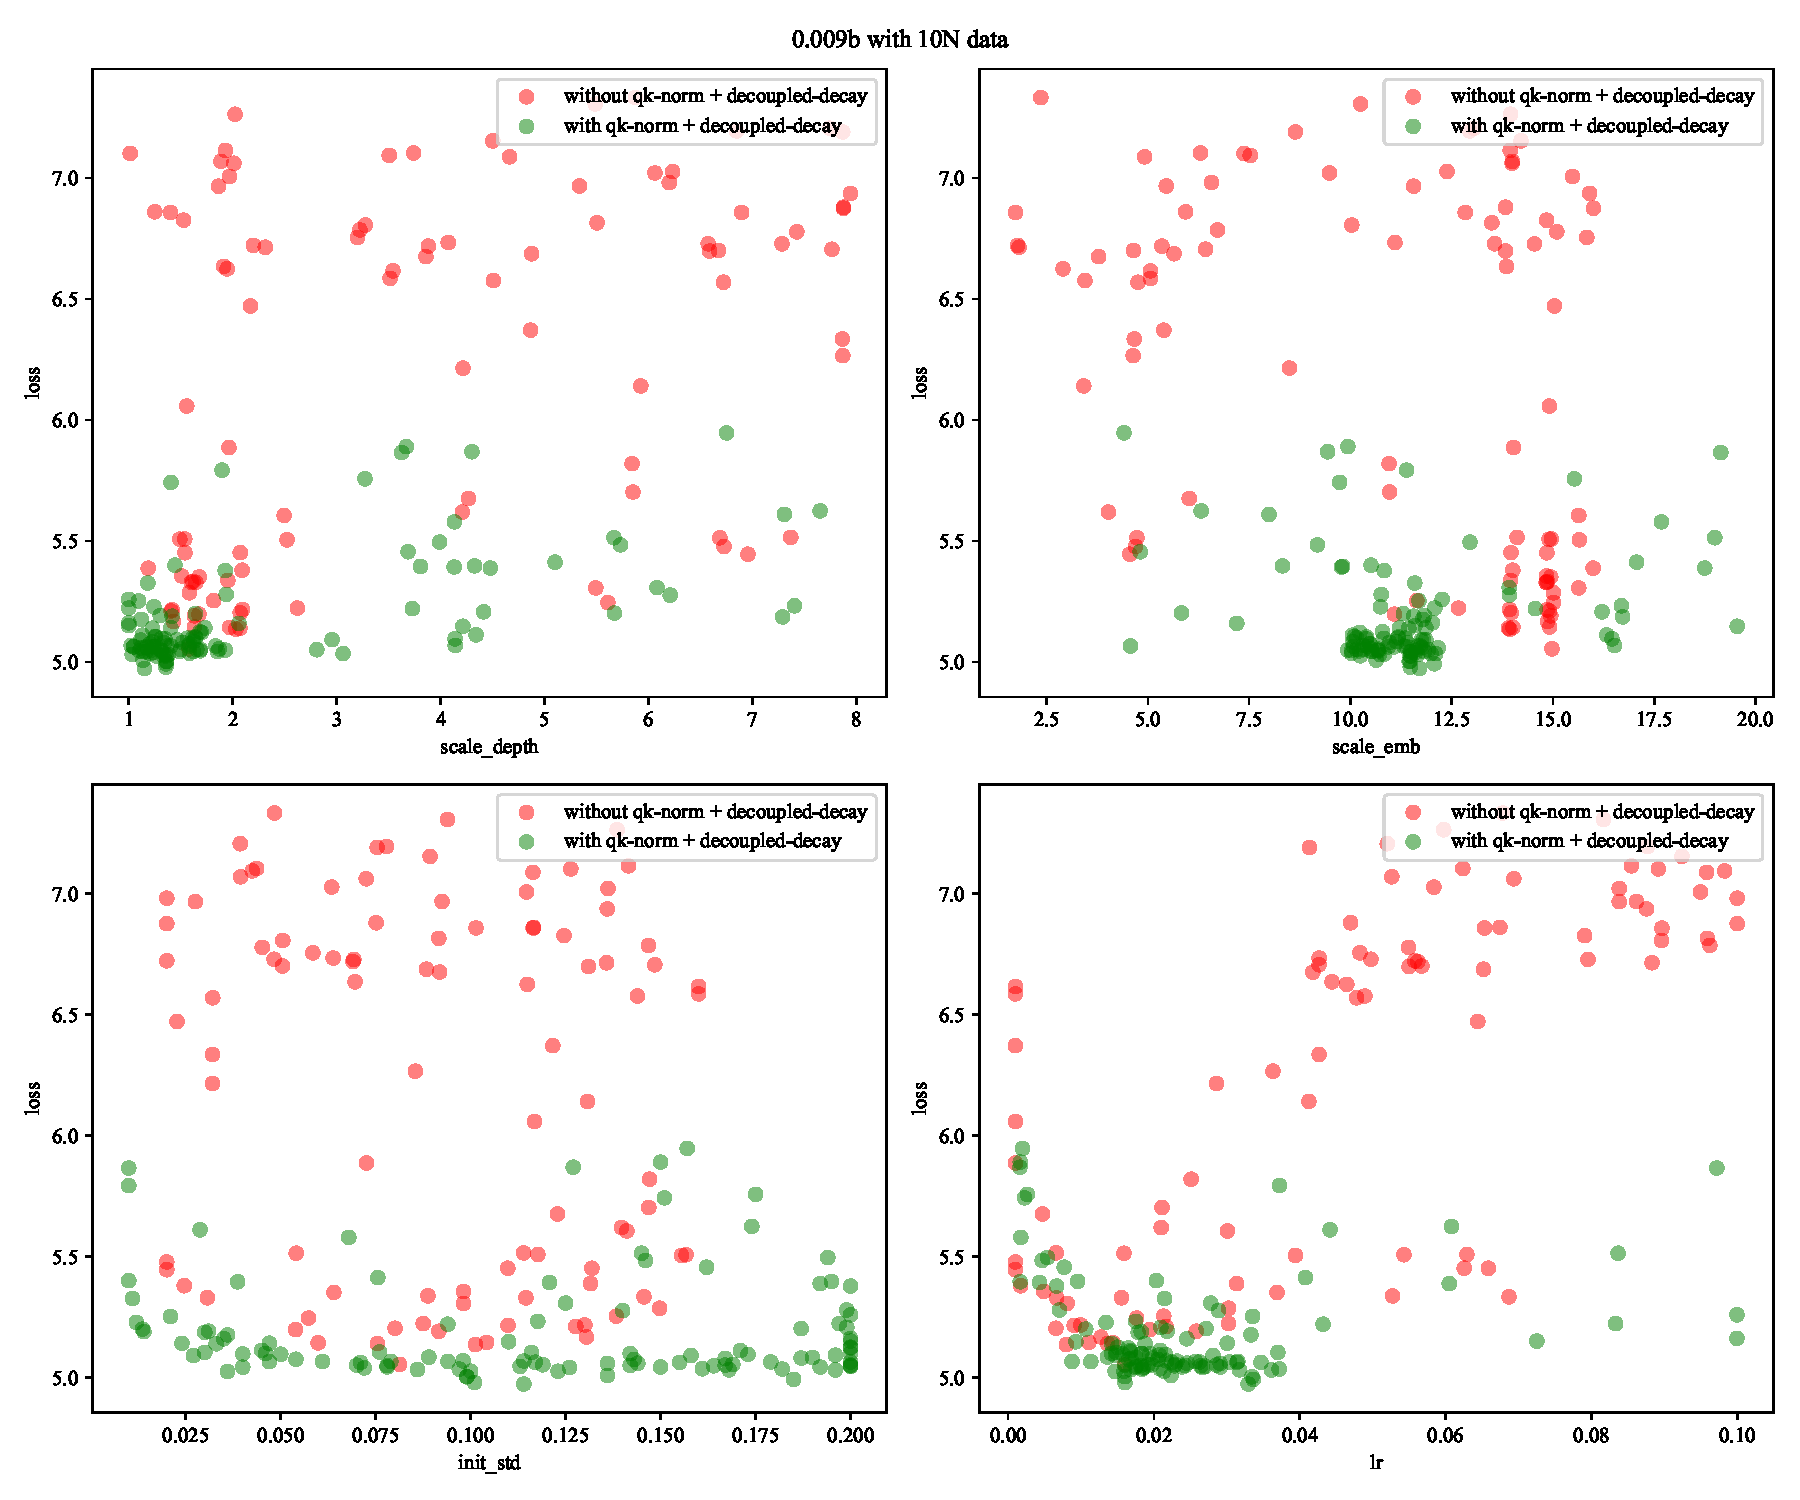
\includegraphics[width=\linewidth]{chap03/mup0.009bwith10Ndata.pdf}
  \caption{Grid search over the $\mu$P parameterization spaces.}
  \label{fig:mupsearch_app}
\end{figure}

\section{最优批量大小}

批量大小决定了模型收敛速度与计算资源消耗之间的平衡。如果批量大小过大,将导致大量的数据和计算成本。另一方面,如果批量大小过小,则需要大量的训练步骤,并且可能导致损失函数的下降有限。我们遵循~\cite{kaplan2020scaling} 从预期损失确定批量大小的方法,并对其设置做了轻微修改。


在~\cite{kaplan2020scaling}中,OpenAI研究了损失函数与token数量之间的关系。在他们的实验中,他们假设消耗更多的步骤等同于消耗更多的时间。在这一假设下,OpenAI定义了一个关键批量大小,该批量大小可以在不消耗过多步骤或token的情况下实现一定的损失。如果实验提供了无限的GPU(至少在实验范围内),这一理由是有效的。由于GPU是无限的,增大批量大小不会增加单步时间,但会减少总步骤数。然而,在我们的实验中,由于我们拥有固定的资源(GPU数量),我们观察到将批量大小翻倍几乎等同于将单步时间翻倍。因此,通过增大批量大小来减少总训练步骤对总训练时间的影响微乎其微。基于这一观察,我们放弃了“不消耗过多步骤”的目标,转而专注于最小化token数量以实现最低损失。

关于最优批量大小与损失之间关系的估计类似于“鸡与蛋”悖论。实际上,通常可以通过初步实验的先验知识对给定模型大小下可实现的损失进行初步估计。然而,未来有可能开发出更精细的估计方法。

最优批量大小和最优学习率可能并不是独立的。为了克服这种相关性,我们首先对学习率进行了初步研究,然后选择一个最优学习率进行批量大小实验,并使用批量大小缩放再次调整学习率。这有点类似于坐标下降优化方法。然而,未来的工作中欢迎更严格的方法。


为实现这一目标,我们分别在 0.09 亿、0.3 亿和 1.7 亿参数规模的模型上进行实验。每个模型规模在全局学习率为 0.01 且使用余弦退火学习率调度器的情况下,在 6 种批量大小下进行训练。我们观察了在 C4~\citep{2019t5} 数据集上最优批量大小随损失的变化趋势(图 \ref{fig:optimalbatchsize} 中的红线)。

\begin {figure}[!htbp]
\centering
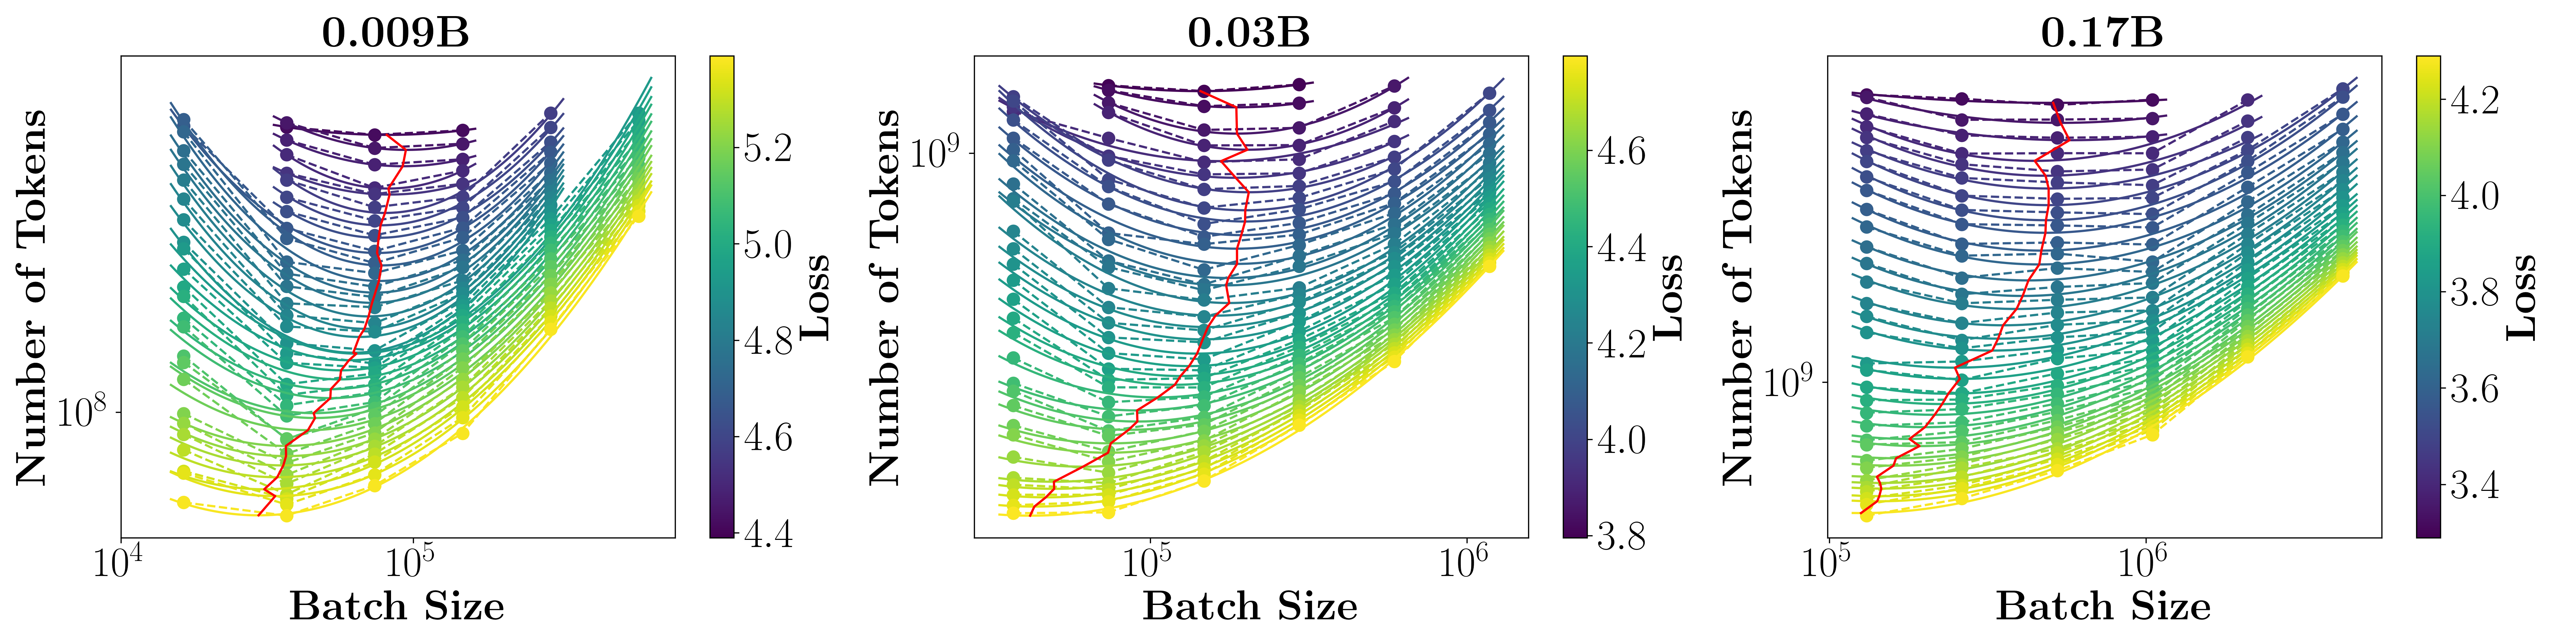
\includegraphics [width=\linewidth]{chap03/batch_size_1.png}
\caption {我们展示了三种不同规模模型在不同批量大小下训练的损失曲线。由具有渐变颜色的点形成的每条垂直线代表一条训练曲线。颜色越浅表示损失越高。}
\label {fig:optimalbatchsize}
\end {figure}


\begin {figure}[!htbp]
\centering
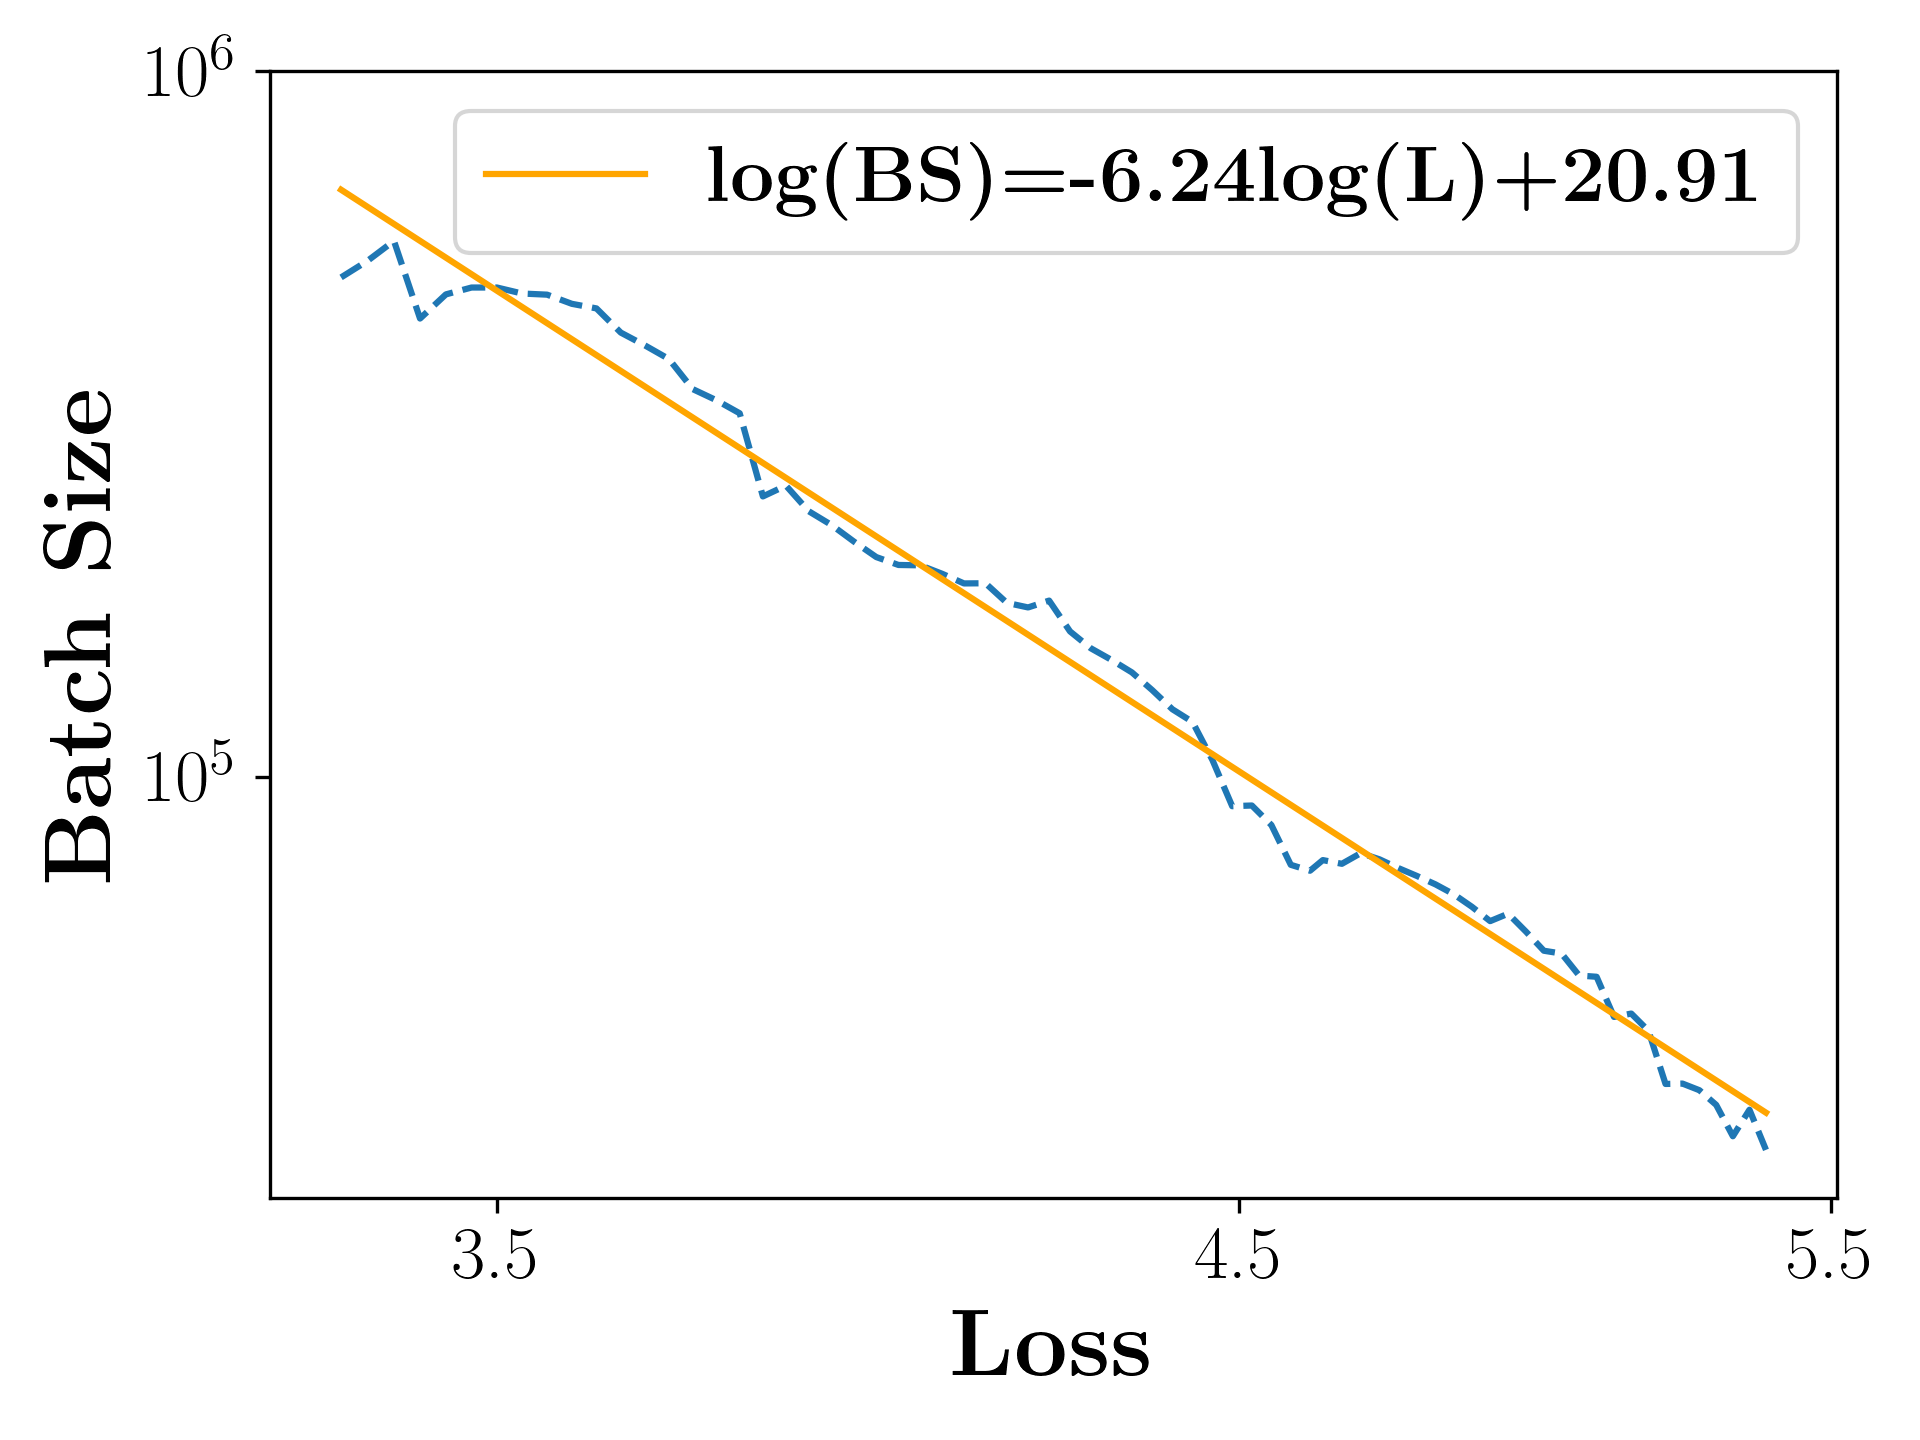
\includegraphics [width=\linewidth]{chap03/batch_size_2.png}
\caption {相连的最优批量大小。 }
\label {fig:optimalbatchsizeconnect}
\end {figure}


如图 \ref {fig:optimalbatchsize} 所示,我们将批量大小绘制在 x 轴上,token 消耗绘制在 y 轴上,点的颜色代表损失。因此,由带颜色的点形成的垂直线表示一条训练曲线。我们使用抛物线拟合等损失点,并用红线连接抛物线的最小值。这些线表明随着损失降低,最优批量大小向更大值移动。然后我们连接这三条线(见图 \ref {fig:optimalbatchsizeconnect}),发现在对数空间中这些线很好地连接成一种线性关系,由此我们得到批量大小与 C4 损失之间的以下关系:$ bs = \frac{1.21\times10^9}{L^{6.24}}$。

\section {最优学习率}
由于我们使用了 Tensor Program~\citep{yang2022tensor, yang2023tensor},我们预计在模型缩放过程中学习率不会发生显著变化。为了验证这一点,我们在 0.4 亿、1 亿、3 亿和 5 亿参数规模上进行了六组学习率实验。在图 \ref {fig:loss_vs_lr} 中,我们发现尽管模型规模增加了十倍,但最优基础学习率 \footnote{二维张量的实际学习率将根据 Tensor Program 进行缩放。} 并没有明显变化,仍保持在 0.01 左右。我们进一步在 21 亿参数规模上进行了简单验证,证实学习率为 0.01 确实能达到最低损失。

\begin{figure}[htbp]
  \centering
  % First minipage for the first figure
      \centering
      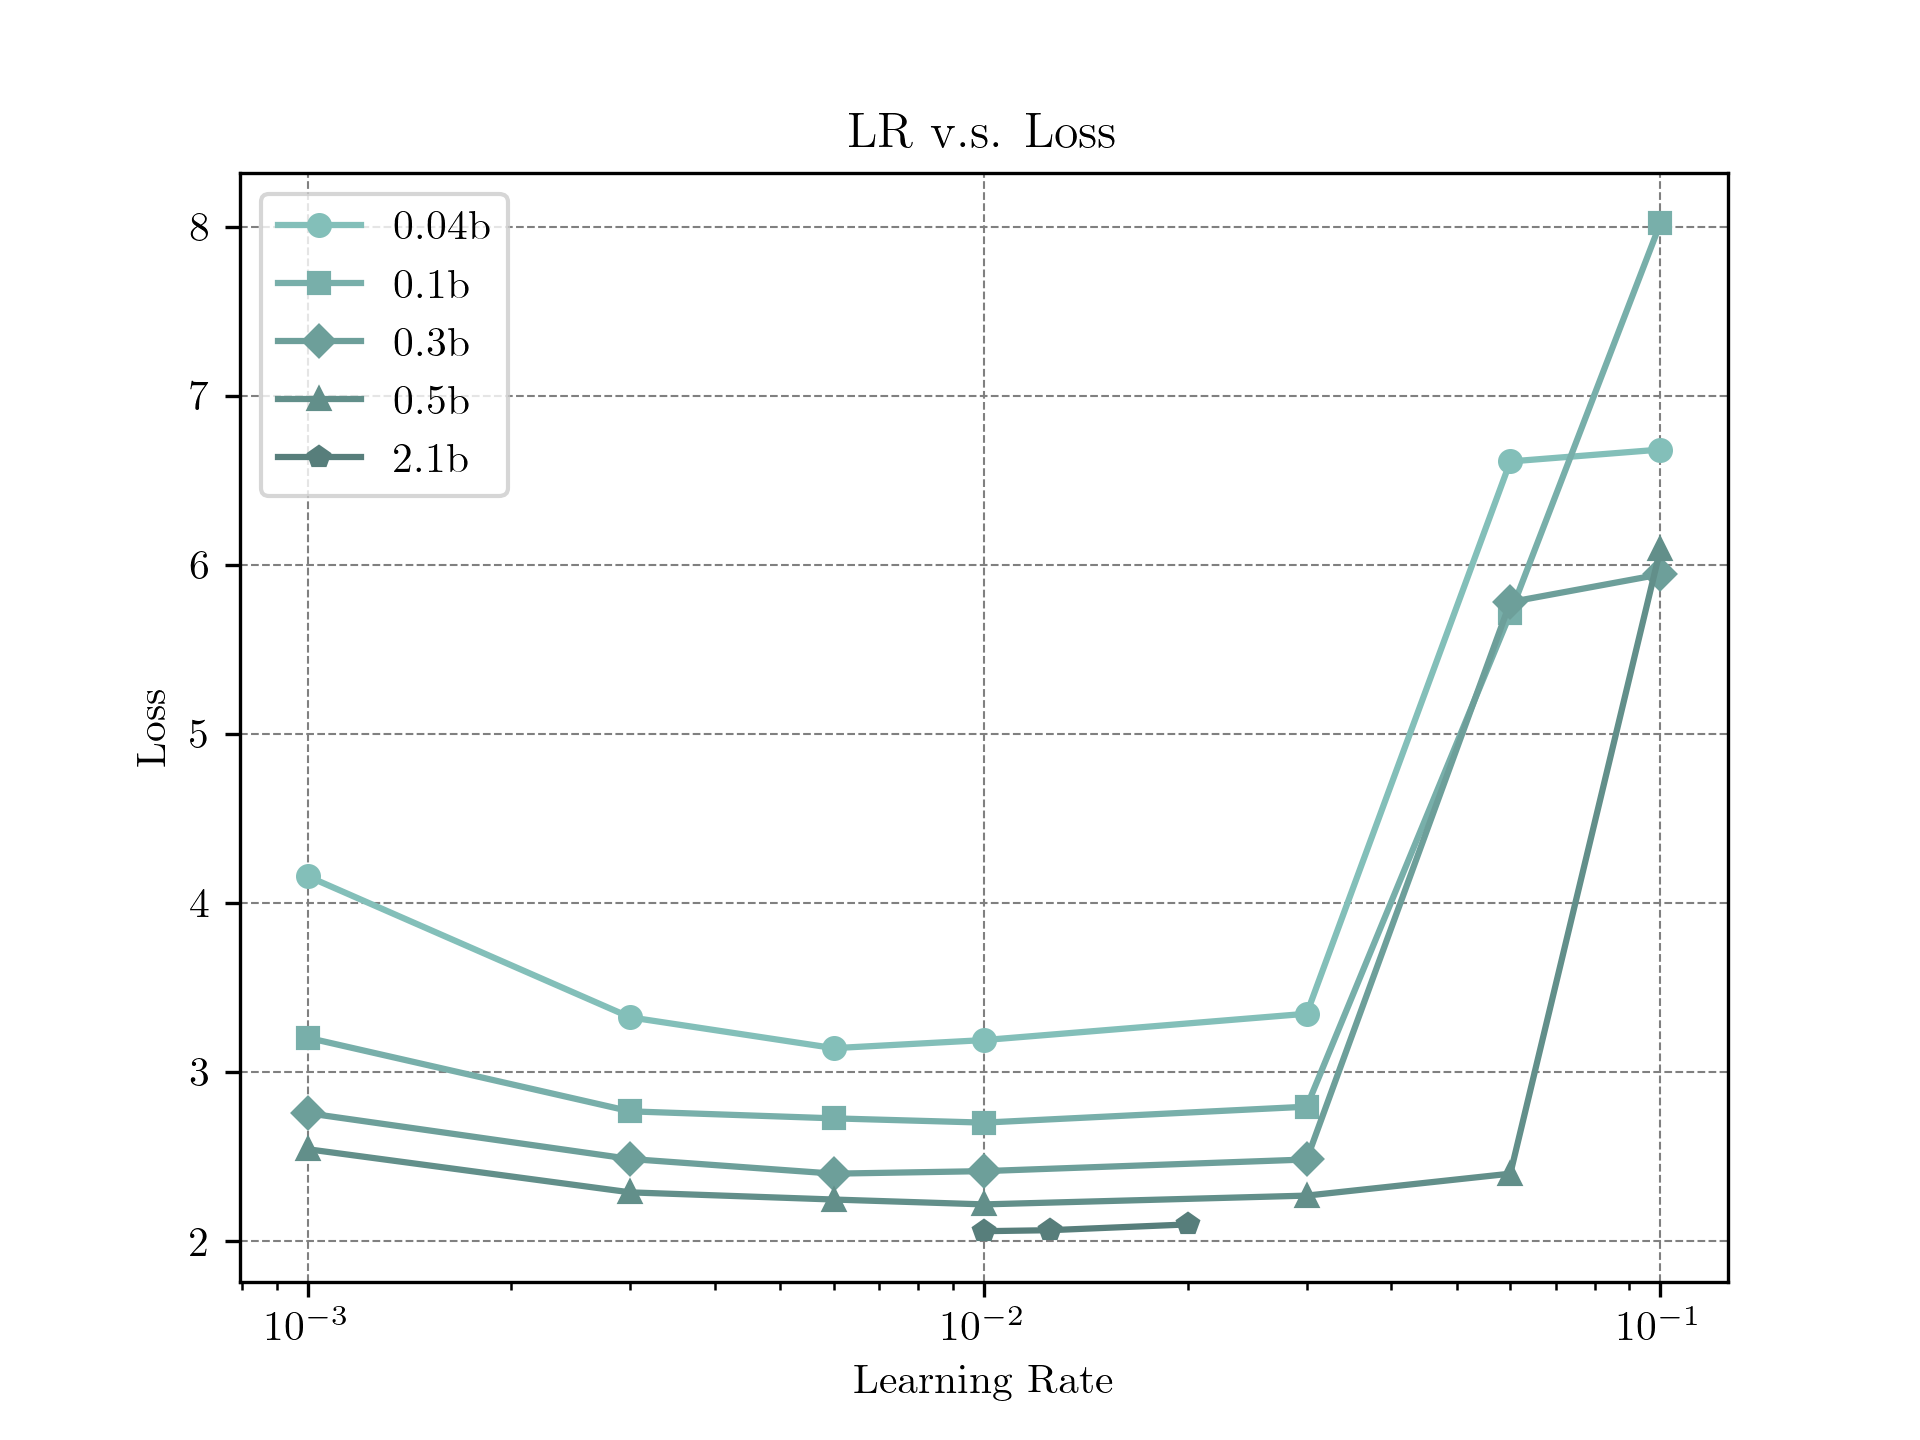
\includegraphics[width=0.9\linewidth]{chap03/loss_vs_lr.png}
      \caption{损失关于学习率的变化图像。在Loss vs Learning Rate. After applying for the Tensor Program, the learning rate shift becomes minimal.}
      \label{fig:loss_vs_lr}
\end{figure}

  % Second minipage for the second figure
%   \begin{minipage}{0.46\linewidth}
%     \centering
%     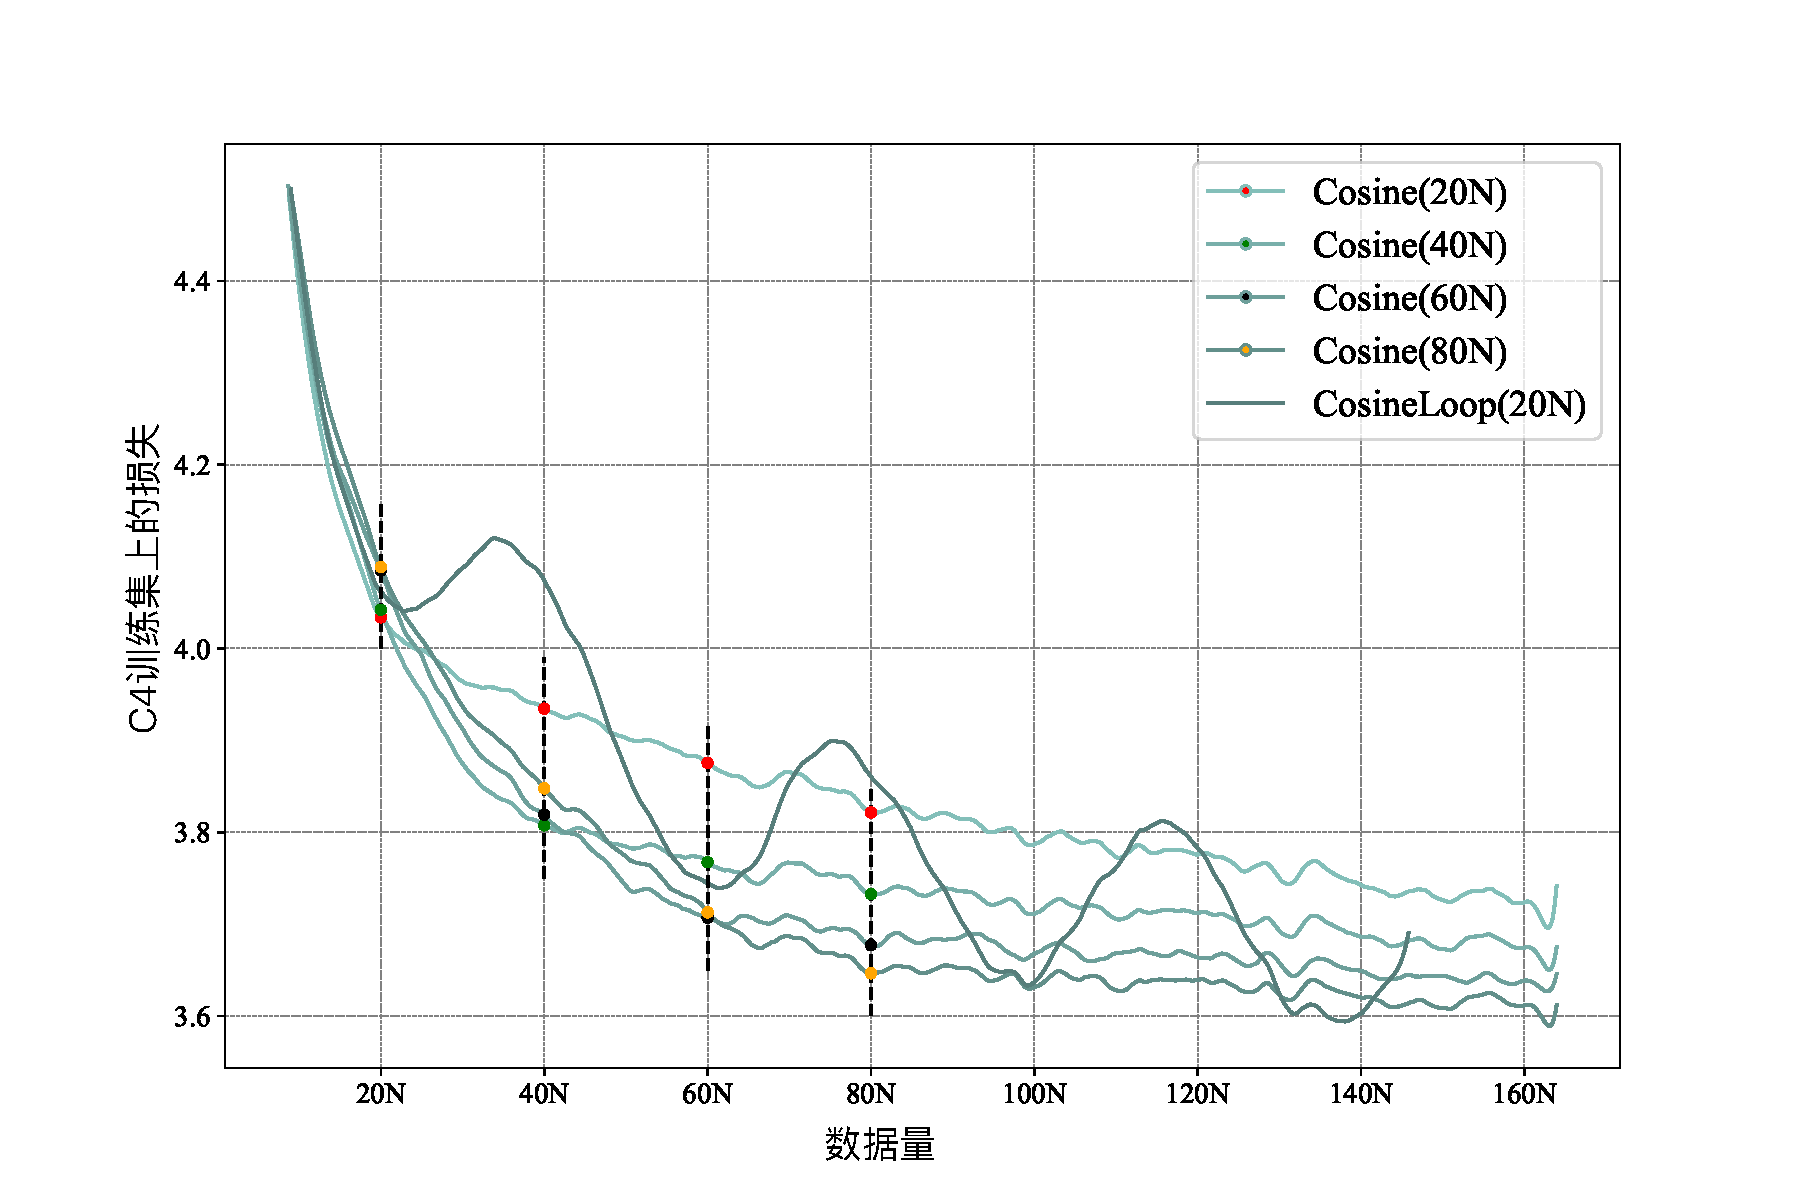
\includegraphics[width=1.0\linewidth]{Fig/cosine_2024-03-26_15-36-16.pdf}
%     \caption{Cosine Learning Rate Scheduler with different periods. The Y-axis is the loss on the C4 corpus.}
%     \label{fig:cosine_lr}
%     \vspace{0.47cm}
% \end{minipage}
% \end{figure}
% \vspace{-5mm}

\section{实验配置}
在表~\ref{tab:appmodel_configs}中列出了在模型规模扩增实验中使用的模型配置。力图让模型的“形状”,即模型宽度与模型深度的比例,尽可能保持一致,以避免任何潜在的性能变化。

\begin{table}[htbp]
    \centering
    \begin{tabular}{c|cccccc}
    \toprule
        \textbf{名称} & \textbf{N (B)}& $d_m$ & $d_{ff}$ &$d_h$ & $n_h$ & $L$ \\
    \midrule
          9M    &  0.009 & 320 & 800 & 64 & 5 & 8\\
           30M &   0.036 & 512 & 1280 & 64 & 8 & 12  \\
          70M &  0.066 & 640 & 1600 & 64 & 10 & 14\\
          0.1B &  0.109 & 768 & 1920 & 64 & 12 & 16  \\
         0.17B &  0.166 & 896 & 2240 & 64 & 14 & 18 \\
         0.2B&  0.241 & 1024 & 2560 & 64 & 16 & 20 \\
        0.5B& 0.499 & 1344 & 3360 & 64 & 21 & 24 \\
    \bottomrule
    \end{tabular}
    \caption{缩放曲线中模型的配置和训练配置。N(B)表示模型的非嵌入参数数量,单位为十亿。
    % BS(M)表示用于训练模型的批次中的token数量(即批量大小),单位为百万。TS表示训练步数。Tokens(B)表示用于训练模型的总token数量。
    }
    \label{tab:appmodel_configs}
\end{table}